% "{'classe':('PSI'),'chapitre':'cin_va','type':('td'),'titre':'Robot de peinture', 'source':'Pôle Chateaubriand - Joliot Curie','comp':(''),'corrige':False}"
%\setchapterimage{fig_00.jpg}
\chapter*{Application \arabic{cptApplication} \\ 
Robot de peinture  \ifnormal $\star$ \else \fi \ifdifficile $\star\star$ \else \fi \iftdifficile $\star\star\star$ \else \fi
 -- \ifprof Corrigé \else Sujet \fi}
\addcontentsline{toc}{section}{Application \arabic{cptApplication} : 
Robot de peinture  \ifnormal $\star$ \else \fi \ifdifficile $\star\star$ \else \fi \iftdifficile $\star\star\star$ \else \fi -- \ifprof Corrigé \else Sujet \fi}

\iflivret \stepcounter{cptApplication} \else
\ifprof  \stepcounter{cptApplication} \else \fi
\fi

\setcounter{question}{0}
\marginnote{Pôle Chateaubriand - Joliot Curie.}
\marginnote[1cm]{
%\UPSTIcompetence[2]{B2-14}
%\UPSTIcompetence[2]{C1-05}
%\UPSTIcompetence[2]{C2-07}
}

\begin{marginfigure}
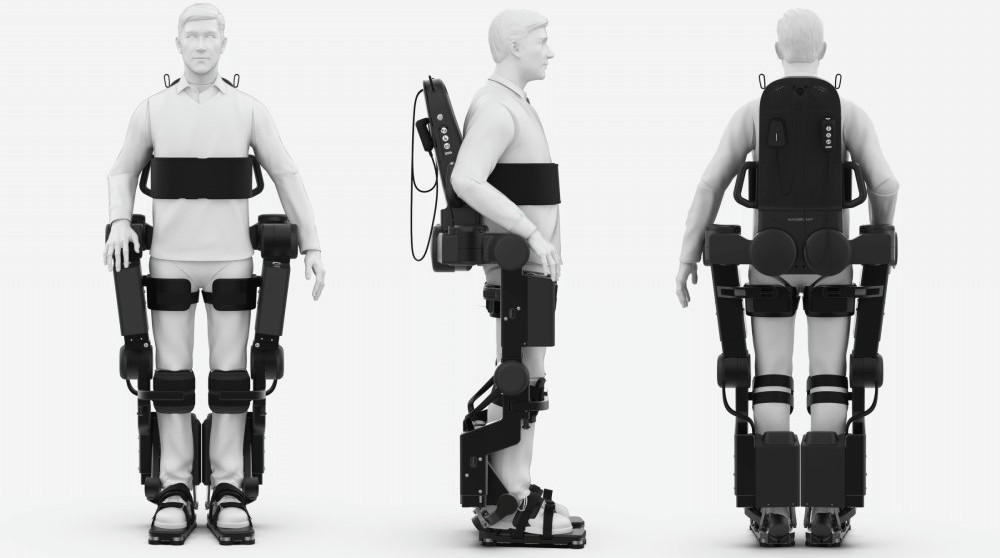
\includegraphics[width=\textwidth]{fig_00}
\end{marginfigure}


\subsection*{Robot de peinture}

\vspace{.25cm}

On étudie un robot de peinture de voiture. Ce robot se déplace par rapport à une carrosserie de voiture, et projette dessus de la peinture. L'objectif est de déterminer les lois du mouvement du robot, pour lui permettre de vérifier le critère de vitesse de déplacement relatif (entre le robot et la carrosserie de voiture) du cahier des charges.

\begin{center}
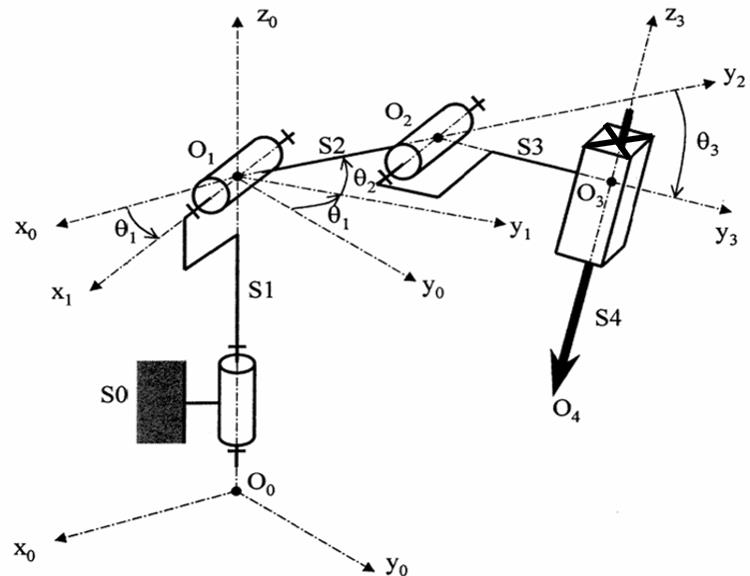
\includegraphics[width=\linewidth]{fig_1}

\end{center}

\vspace{.25cm}


La modélisation cinématique du robot est donnée sur la figure suivante :


\begin{center}
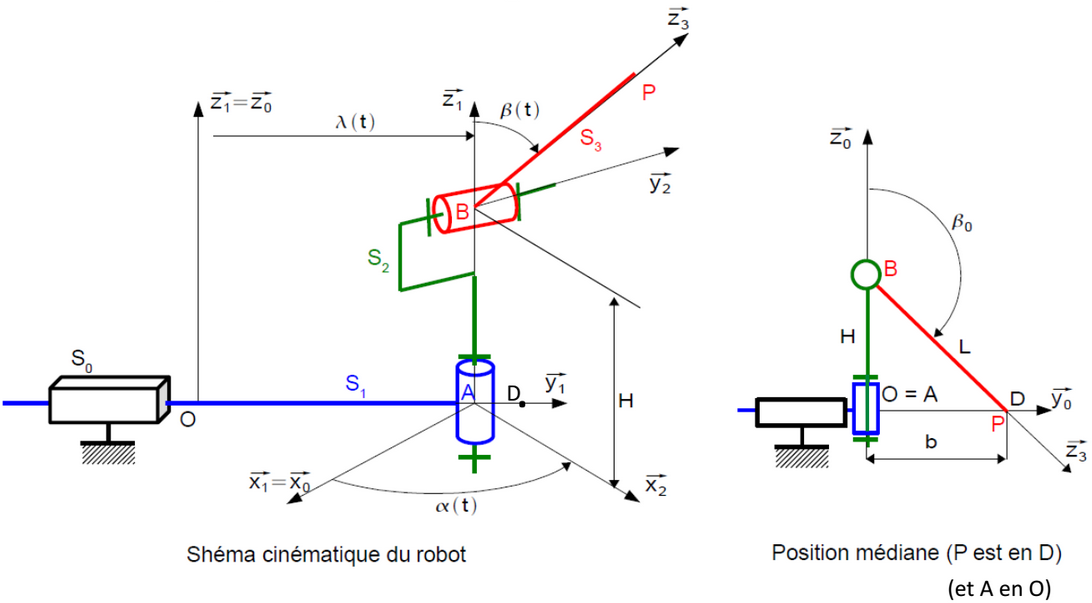
\includegraphics[width=\linewidth]{fig_2}
\end{center}



\vspace{.25cm}

Le chariot $S_1$, auquel on associe le repère $\mathcal{R}_1\left(A,\vect{x_1},\vect{y_1},\vect{z_1}\right)$ est en mouvement de translation de direction $\vect{y_0}$ par rapport au bâti $S_0$ de repère $\mathcal{R}_0\left(A,\vect{x_0},\vect{y_0},\vect{z_0}\right)$. 

Le corps $S_2$, auquel on associe le repère $\mathcal{R}_2\left(A,\vect{x_2},\vect{y_2},\vect{z_2}\right)$ est en mouvement de rotation autour de l'axe $(B,\vect{z_0})$ avec le chariot $S_1$. 

Le bras $S_3$, auquel on associe le repère $\mathcal{R}_3\left(B,\vect{x_3},\vect{y_3},\vect{z_3}\right)$ est en mouvement de rotation autour de l'axe $(B,\vect{y_2})$ avec le corps $S_2$. 





\question{Construire les figures planes de repérage/paramétrage.} 

\question{Exprimer les vecteurs vitesse instantanée de rotation $\vecto{1}{0}$, $\vecto{2}{1}$, $\vecto{3}{2}$ et $\vecto{3}{0}$.}

\question{Déterminer $\vectv{P}{3}{0}$.}

\question{Déterminer $\vectg{P}{3}{0}$.}

\question{Déterminer $\vectg{P}{3}{0}\cdot\vect{x_0}$.}

\question{Calculer les produits vectoriels et scalaires suivants : $\vect{z_3}\wedge \vect{x_2}$ et $\vect{z_3}\cdot \vect{x_2}$,  $\vect{z_3}\wedge \vect{y_1}$ et $\vect{z_3}\cdot \vect{y_1}$.}


On a $\vect{OD}=b\vect{y_0}$ avec $b=\sqrt{L^2-H^2}$.
On désire que $P$ décrive la droite $(D,\vect{x_0})$ à vitesse constante $V$, conformément au cahier des charges. 

\question{Représenter sur une figure dans le plan $(O,\vect{x_0},\vect{y_0})$, puis sur une figure dans le plan $(O,\vect{x_0},\vect{y_0})$, les positions des points $O$, $D$, $A$, $B$ et $P$ du robot lorsque celui-ci est en position extrême ($A$ est en $D$).}


\ifprof
\else
\begin{marginfigure}
\centering

\includegraphics[width=3cm]{Cy_12_Ch_03_Application_04_RobotPeinture_qr}
\end{marginfigure}
\fi

\question{Traduire, à l'aide de l'expression de $\vectv{P}{3}{0}$ le fait que $P$ se déplace à la vitesse $V$ selon $\vect{x_0}$. En déduire $\dot{\beta}$.}

\question{Exprimer alors $\dot{\lambda}$ et $\dot{\alpha}$ en fonction de $L$, $V$, $\alpha$ et $\beta_0$. }

\question{A l'aide de la figure précédente, exprimer $\beta_0$ en fonction de $b$ et $L$.}

\question{Exprimer $\dot{\lambda}$ et $\dot{\alpha}$ en fonction de $V$, $b$ et $\alpha$.}

